% Team study guide: explains the whole project part by part.
% Build:  cd presentation/guide && latexmk -pdf guide.tex
\documentclass[11pt,a4paper]{article}
\usepackage[margin=2.3cm]{geometry}
\usepackage{lmodern}
\usepackage[T1]{fontenc}
\usepackage{microtype}
\usepackage{amsmath,amssymb}
\usepackage{graphicx}
\usepackage{booktabs}
\usepackage{array}
\usepackage{enumitem}
\usepackage{xcolor}
\usepackage{tikz}
\usetikzlibrary{arrows.meta,positioning,calc}
\usepackage[most]{tcolorbox}
\usepackage{fancyhdr}
\usepackage{titlesec}
\usepackage[colorlinks,allcolors=blue!55!black]{hyperref}
\usepackage[capitalize,nameinlink]{cleveref}

\definecolor{navy}{HTML}{14213D}
\definecolor{accent}{HTML}{2A78D6}
\definecolor{warm}{HTML}{EB6834}
\titleformat{\section}{\Large\bfseries\color{navy}}{\thesection}{0.6em}{}
\titleformat{\subsection}{\large\bfseries\color{navy}}{\thesubsection}{0.5em}{}
\setlist{itemsep=2pt,topsep=3pt}
\setlength{\parskip}{4pt}

\newtcolorbox{idea}[1][Key idea]{colback=accent!6,colframe=accent,fonttitle=\bfseries,title=#1,boxrule=0.6pt,arc=2pt,left=6pt,right=6pt}
\newtcolorbox{say}[1][Say it like this]{colback=black!3,colframe=black!45,fonttitle=\bfseries,title=#1,boxrule=0.6pt,arc=2pt,left=6pt,right=6pt}
\newtcolorbox{careful}[1][Be careful]{colback=warm!7,colframe=warm,fonttitle=\bfseries,title=#1,boxrule=0.6pt,arc=2pt,left=6pt,right=6pt}

\pagestyle{fancy}
\fancyhf{}
\lhead{\small\color{black!60}Face Symmetry Measurement: team study guide}
\rhead{\small\color{black!60}EE604, IIT Kanpur}
\cfoot{\small\thepage}

% the same auto-generated numbers that the paper uses
% Auto-generated by experiments/make_tables.py -- do not edit by hand
\newcommand{\rhoMzero}{0.823}
\newcommand{\rhoMzeroNoAlign}{0.614}
\newcommand{\rhoMzeroFixed}{0.931}
\newcommand{\rhoMone}{0.938}
\newcommand{\rhoMthree}{0.947}
\newcommand{\maeMone}{0.45}
\newcommand{\maeMthree}{0.45}
\newcommand{\kdWrong}{58.3}
\newcommand{\nmeFitInner}{3.95}
\newcommand{\nmeHandInner}{4.23}
\newcommand{\nmeFitJaw}{8.13}
\newcommand{\nmeHandJaw}{10.11}
\newcommand{\nmeFitInnerMed}{3.13}
\newcommand{\shrinkGlobal}{12.4}
\newcommand{\shrinkMouth}{26.7}
\newcommand{\shrinkBrows}{1.9}
\newcommand{\pBrows}{0.08}
\newcommand{\silentCleanOne}{5.8}
\newcommand{\silentCleanTwo}{4.9}
\newcommand{\silentCleanThree}{4.0}
\newcommand{\covCleanThree}{89.7}
\newcommand{\accCleanThree}{42.0}
\newcommand{\silentPoolOne}{8.1}
\newcommand{\silentPoolTwo}{3.4}
\newcommand{\silentPoolThree}{3.6}
\newcommand{\covPoolThree}{63.2}
\newcommand{\accPoolThree}{21.0}
\newcommand{\silentBlurOne}{14.4}
\newcommand{\silentBlurTwo}{2.7}
\newcommand{\silentBlurThree}{2.3}
\newcommand{\covBlurThree}{35.6}
\newcommand{\accBlurThree}{5.2}
\newcommand{\silentDownOne}{9.2}
\newcommand{\silentDownTwo}{1.8}
\newcommand{\silentDownThree}{1.9}
\newcommand{\covDownThree}{33.4}
\newcommand{\accDownThree}{4.0}
\newcommand{\driftPoolOne}{0.076}
\newcommand{\driftPoolThree}{0.054}
\newcommand{\driftPoolZero}{0.070}
\newcommand{\driftReduction}{29}
\newcommand{\rotNoAlignMax}{3.67}
\newcommand{\rotMthreeMax}{0.052}
\newcommand{\detBlurEight}{79.0}
\newcommand{\detMin}{79.0}
\newcommand{\rhoYawRef}{0.91}
\newcommand{\rhoYawRefAcc}{0.75}
\newcommand{\rhoYawMthree}{0.96}
\newcommand{\yawLow}{1.20}
\newcommand{\yawHigh}{5.50}
\newcommand{\rhoMirrorNme}{0.59}
\newcommand{\aurcRandom}{3.37}
\newcommand{\aurcMirror}{2.99}
\newcommand{\aurcGateTwo}{3.29}
\newcommand{\aurcOracle}{2.75}
\newcommand{\gapClosed}{61}
\newcommand{\aurcAsymRandom}{0.442}
\newcommand{\aurcAsymMirror}{0.418}
\newcommand{\aurcAsymGate}{0.437}
\newcommand{\rhoMirrorErr}{0.03}
\newcommand{\pAccept}{42.0}
\newcommand{\pCaution}{47.8}
\newcommand{\pReject}{10.3}
\newcommand{\nmeAccept}{3.03}
\newcommand{\nmeCaution}{4.71}
\newcommand{\occEye}{0.9}
\newcommand{\occNose}{17.5}
\newcommand{\occNoseOther}{8.5}
\newcommand{\occMouth}{18.4}
\newcommand{\occMouthOther}{2.2}
\newcommand{\alphaIndex}{0.467}
\newcommand{\trainMedian}{2.14}
\newcommand{\runtime}{46}
\newcommand{\nTrainOk}{810}

\graphicspath{{../../results/figures/}}
\renewcommand{\cite}[1]{}  % the paper's tables cite the baseline; no bibliography here

\begin{document}

\begin{center}
{\Huge\bfseries\color{navy} Face Symmetry Measurement}\\[6pt]
{\Large Understanding the whole project, part by part}\\[10pt]
{\large A study guide for presenting and defending the project}\\[8pt]
Ankit Yadav (230150) \quad Ashish Porwal (230229) \quad Mahi Mittal (230617)\\
Pankaj Kumar (230733) \quad Prutha Vinay (230807)\\[4pt]
EE604 Image Processing, IIT Kanpur, November 2026
\end{center}

\vspace{4pt}
\begin{idea}[How to use this guide]
Everyone should read \textbf{Part 1} (the one-page summary) and \textbf{Part 9} (questions).
Each part then stands on its own: read the parts for the slides you present. All numbers
are produced by the project's scripts and are identical to those in the paper and slides.
Boxes marked \emph{Say it like this} give wording you can use in the presentation;
boxes marked \emph{Be careful} list claims you must \emph{not} make.
\end{idea}

\tableofcontents
\newpage

%======================================================================
\section{The project in one page}
%======================================================================

\textbf{What it does.} You give the system one photo of a face. It finds points on the
face (eye corners, nose, mouth, jaw\dots), compares the left half with the mirror image of
the right half, and reports how far the face is from perfectly mirror-symmetric. Before it
reports anything, it checks whether the photo is good enough. It answers \textbf{accept},
\textbf{caution} or \textbf{reject}, and explains why.

\textbf{Input:} one RGB photo containing a face.\\
\textbf{Output:} accept/caution/reject with reasons; a global asymmetry number $A$ (in \% of the
eye-corner distance); values for brows, eyes, nose, mouth and jaw; a stability band; pictures
(overlays); a CSV/JSON export.\\
\textbf{Constraints:} 2D image only, no model training, runs on a laptop CPU
(\runtime\,ms per image), and it is \emph{not} a medical, beauty or identity score.

\textbf{Why it is needed.} Existing tools always return a number, even for photos that cannot
support one. We found that on ordinary in-the-wild photos the measured asymmetry follows how
far the head is turned almost perfectly ($\rho$ = \rhoYawRef{}), even when the points are
placed by human experts. Without a check, a ``symmetry score'' of a selfie mostly measures
head pose.

\textbf{Our four contributions.}
\begin{enumerate}
\item \textbf{Correct pairs and a fitted mirror line.} Each point is compared with its true
anatomical twin, and the mirror line is estimated rather than assumed vertical. The older
nearest-neighbour (KD-tree) matching picks the wrong twin \kdWrong\% of the time.
\item \textbf{The mirror test.} We run the detector on the photo \emph{and} on its mirror
image. A face's asymmetry cannot change when the photo is flipped, so if the two results
disagree, the landmarks are unreliable. This needs no ground truth.
\item \textbf{A quality and pose gate} with seven signals, whose thresholds were fixed a priori
or learned on training images only.
\item \textbf{A way to evaluate without symmetry labels:} compare with the same measurement
made from expert-placed landmarks, and degrade photos in 26 controlled ways.
\end{enumerate}

\begin{center}
\begin{tabular}{@{}lc@{}}
\toprule
Headline result (LFPW test set) & Value\\
\midrule
Agreement with expert-landmark reference, baseline $\rightarrow$ ours (Spearman $\rho$) & \rhoMzero{} $\rightarrow$ \rhoMthree{}\\
Wrong partners chosen by the baseline's KD-tree matching & \kdWrong\%\\
Mirror test vs.\ true landmark error (Spearman $\rho$) & \rhoMirrorNme{}\\
Silent failures on degraded photos, no gate $\rightarrow$ full system & \silentPoolOne\% $\rightarrow$ \silentPoolThree\%\\
Score drift reduction from mirror averaging & \driftReduction\%\\
Head yaw vs.\ asymmetry, even from expert landmarks (Spearman $\rho$) & \rhoYawRef{}\\
\bottomrule
\end{tabular}
\end{center}

\begin{say}
``Existing symmetry tools always give you a number. Ours first checks whether the photo can
support a measurement, verifies its own landmarks with a mirror test, and measures with
the correct anatomical pairs and a fitted symmetry axis. We evaluated it against expert
landmarks and under 26 controlled degradations.''
\end{say}

%======================================================================
\section{Background you need}
%======================================================================

\subsection{Facial landmarks}
A \textbf{landmark} is a named point on the face, such as ``outer corner of the left eye''
or ``tip of the nose''. A \textbf{landmark detector} is a pretrained model that finds these
points in a photo.

\begin{itemize}
\item \textbf{The 68-point layout} (iBUG / 300-W) is the standard layout of academic
benchmarks: 17 jaw points, 10 eyebrow points, 9 nose points, 12 eye points and 20 mouth
points. Human experts annotated thousands of photos with it. That is why we report our
results in this layout: we can compare against the experts.
\item \textbf{MediaPipe Face Landmarker} (Google) finds 478 points, a dense mesh covering the
whole face (468 face points + 10 iris points). It runs in real time on a CPU and also outputs
a $4\times4$ \emph{transformation matrix} that tells us the head's rotation.
\item \textbf{The canonical face model} is MediaPipe's ``average face'' in 3D, with the same 468
vertices. It is \emph{exactly} left--right symmetric. We use this fact to know which vertex
is the mirror twin of which (\cref{sec:perm}).
\end{itemize}

\subsection{What ``symmetric'' means geometrically}
A face is mirror-symmetric if there is a line (the \textbf{symmetry axis} or \textbf{midline})
such that reflecting the left half across it lands exactly on the right half.
\begin{itemize}
\item \textbf{Bilateral pairs}: points that have a twin on the other side (left eye
corner $\leftrightarrow$ right eye corner).
\item \textbf{Midline points}: points that are their own twin (nose tip, chin, centre of the lips).
\item \textbf{Asymmetry}: how far a point is from where the mirror image of its twin says it
should be.
\end{itemize}

\begin{center}
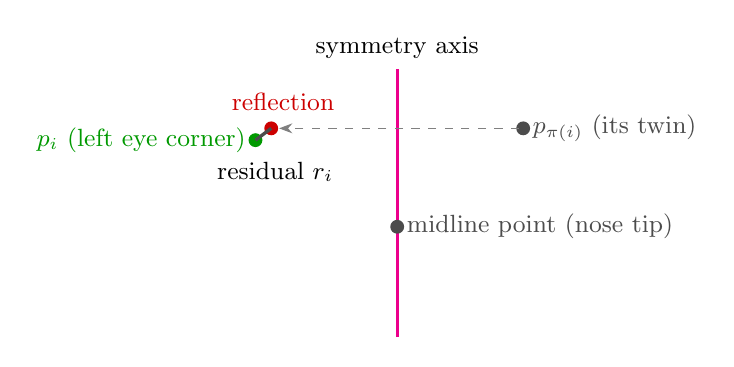
\begin{tikzpicture}[scale=1.0,>=Stealth]
\draw[magenta,very thick] (0,-1.6) -- (0,1.8) node[above,black]{\small symmetry axis};
\fill[green!60!black] (-1.8,0.9) circle (2.5pt) node[left]{\small $p_i$ (left eye corner)};
\fill[black!70] (1.6,1.05) circle (2.5pt) node[right]{\small $p_{\pi(i)}$ (its twin)};
\fill[red!80!black] (-1.6,1.05) circle (2.5pt);
\draw[->,dashed,black!50] (1.55,1.05) -- (-1.5,1.05);
\node[red!80!black,above] at (-1.45,1.15) {\small reflection};
\draw[very thick,black!70] (-1.8,0.9) -- (-1.6,1.05);
\node[below] at (-1.55,0.75) {\small residual $r_i$};
\fill[black!70] (0,-0.2) circle (2.5pt) node[right]{\small midline point (nose tip)};
\end{tikzpicture}
\end{center}
The \textbf{residual} $r_i$ is the small gap between a point and the reflection of its twin.
For a perfectly symmetric face every residual is zero.

\subsection{Normalisation: why ``\% IOD''}
Distances in pixels depend on image size: a face photographed close up has bigger
gaps. We divide every distance by the \textbf{inter-ocular distance (IOD)}, the distance
between the two outer eye corners. It is the standard normaliser of the 300-W benchmark. An
asymmetry of ``2\% IOD'' means ``2\% of the distance between the outer eye corners''. On an adult face that distance is roughly 9\,cm, so
2\% IOD is just under 2\,mm.

\subsection{Head pose: yaw, pitch and roll}
\begin{itemize}
\item \textbf{Roll}: tilting the head towards a shoulder (in-plane rotation). A 2D rotation
can undo it, and our fitted axis is unaffected by it.
\item \textbf{Yaw}: turning the head left or right (shaking ``no''). One half of the face
gets foreshortened in the photo, and \emph{no 2D operation can undo that}.
\item \textbf{Pitch}: nodding up or down. It distorts vertical proportions.
\end{itemize}
This is the core limitation of any 2D symmetry measurement, and the reason the gate checks
yaw and pitch.

\subsection{Statistics used in the results}
\begin{itemize}
\item \textbf{Spearman $\rho$} (rank correlation): do two measurements put the faces in the
same order? 1 = identical order, 0 = unrelated. It works even when the two measurements use
different units, which is why we use it to compare the baseline (face-width units) with ours
(IOD units).
\item \textbf{Pearson $r$}: linear correlation.
\item \textbf{MAE} (mean absolute error): the average of $|A_{\text{ours}}-A_{\text{ref}}|$, in \% IOD.
\item \textbf{NME} (normalised mean error): the average distance between detected and
expert landmarks, divided by IOD. The standard landmark-accuracy metric.
\item \textbf{Wilcoxon test}: a paired test of whether one measurement is systematically
larger than another.
\end{itemize}

%======================================================================
\section{The baseline we improve on (M0)}
%======================================================================
The closest public tool is \texttt{nashokan/FacialAsymmetry} on GitHub. It implements the
symmetry part of Varghaei et al.\ (ICCV Workshops 2025). Since the repository has \textbf{no
licence}, we did not copy its code; we \textbf{re-implemented its method} from its description.
Its steps are:
\begin{enumerate}
\item Detect the 478 MediaPipe points.
\item Align the face: rotate and scale the image so that vertices 33 and 263 sit at fixed
positions, then detect again.
\item Take a vertical midline at the average $x$ of vertices 33 and 263.
\item Reflect every point on the left of the midline, and match it to the \emph{nearest}
right-side point (KD-tree nearest-neighbour search).
\item Report the mean matched distance divided by face width.
\end{enumerate}

\textbf{Its three problems, which we measured:}
\begin{enumerate}
\item \textbf{Wrong partners.} The mesh is dense, so the nearest point after reflection is
often a \emph{neighbour} of the true twin. The matching then absorbs part of the asymmetry it
should measure. On LFPW, \kdWrong\% of matches are the wrong anatomical twin
(\cref{fig:corr}).
\item \textbf{Assumed vertical midline.} Any tilt of the head, or any error in vertices 33/263,
looks like asymmetry. Without the alignment step the baseline's agreement drops from
\rhoMzero{} to \rhoMzeroNoAlign{}.
\item \textbf{No quality check.} It always returns a number.
\end{enumerate}
(Detail worth knowing: vertices 33 and 263 are the \emph{outer} eye corners, although the
baseline's code comments call them inner corners.)

\begin{figure}[h]
\centering
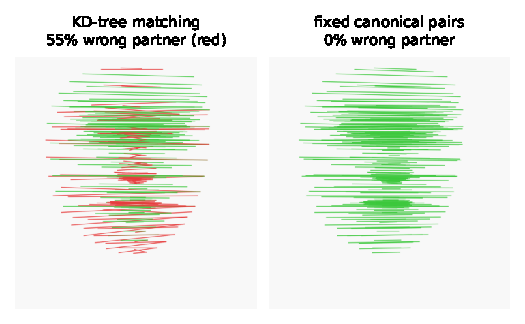
\includegraphics[width=0.6\linewidth]{correspondence.pdf}
\caption{Matches for one face (geometry only). Left: KD-tree matching; red lines are wrong
partners. Right: our fixed anatomical pairs.}
\label{fig:corr}
\end{figure}

%======================================================================
\section{Our method, step by step}
%======================================================================

\begin{figure}[h]
\centering
\resizebox{\linewidth}{!}{%
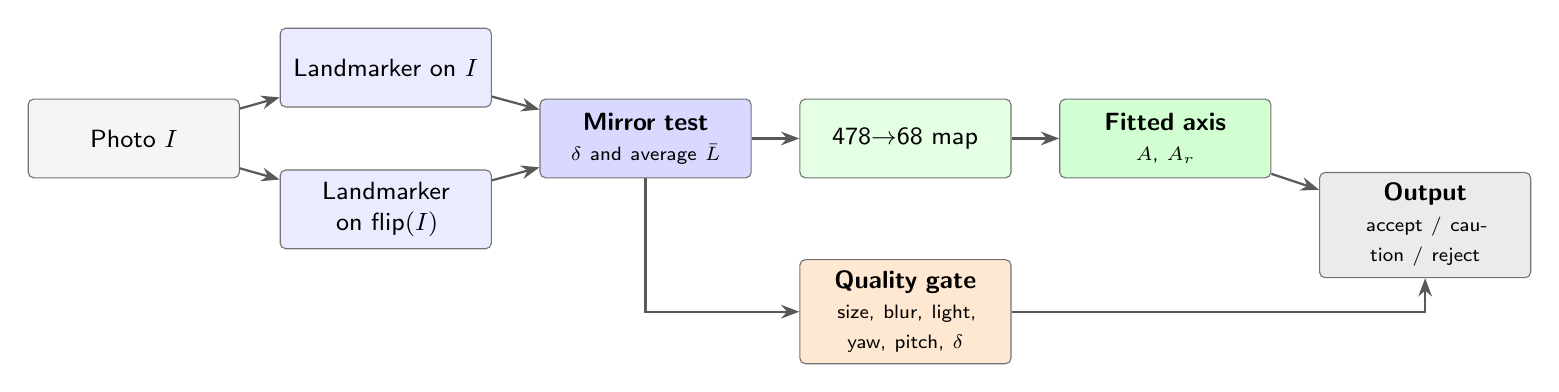
\begin{tikzpicture}[font=\sffamily\small,>=Stealth,
  box/.style={draw=black!55,rounded corners=2pt,fill=#1,align=center,inner sep=4pt,minimum height=1.0cm,text width=2.4cm},
  box/.default=white, arr/.style={->,thick,black!65}]
\node[box=black!4] (in) at (0,0) {Photo $I$};
\node[box=blue!8] (d1) at (3.2,0.9) {Landmarker on $I$};
\node[box=blue!8] (d2) at (3.2,-0.9) {Landmarker on flip$(I)$};
\node[box=blue!15] (mt) at (6.5,0) {\textbf{Mirror test}\\\scriptsize $\delta$ and average $\bar L$};
\node[box=green!10] (map) at (9.8,0) {478$\to$68 map};
\node[box=green!18] (ax) at (13.1,0) {\textbf{Fitted axis}\\\scriptsize $A$, $A_r$};
\node[box=orange!18] (gate) at (9.8,-2.2) {\textbf{Quality gate}\\\scriptsize size, blur, light, yaw, pitch, $\delta$};
\node[box=black!8] (out) at (16.4,-1.1) {\textbf{Output}\\\scriptsize accept / caution / reject};
\draw[arr] (in) -- (d1); \draw[arr] (in) -- (d2);
\draw[arr] (d1) -- (mt); \draw[arr] (d2) -- (mt);
\draw[arr] (mt) -- (map); \draw[arr] (map) -- (ax);
\draw[arr] (mt) |- (gate); \draw[arr] (ax) -- (out); \draw[arr] (gate) -| (out);
\end{tikzpicture}}
\caption{The full system (variant M3). The numbered steps below follow this picture.}
\end{figure}

\subsection{Step 1: detect landmarks (\texttt{detector.py})}
\textbf{What:} run MediaPipe Face Landmarker on the photo. We get 478 points in pixel
coordinates and the transformation matrix, from which we read yaw, pitch and roll.\\
\textbf{Why MediaPipe:} it is pretrained (no training needed), fast on a CPU, and its mesh has
a \emph{fixed topology}: vertex 33 is always the same anatomical spot, on every face. That
is what makes fixed pairs possible.\\
\textbf{Limitation:} it gives no confidence per landmark (the \texttt{visibility} field is empty).
The mirror test (Step 5) fills this gap.

\subsection{Step 2: find each point's mirror twin (\texttt{mesh.py})}\label{sec:perm}
\textbf{What:} take the canonical face model, flip it ($x\to -x$), and for each vertex find the
vertex that lands in its place. Because the canonical model is exactly symmetric, this
match is perfect (error 0). It gives a \textbf{mirror permutation} $\pi$: $\pi(i)$ is the
twin of vertex $i$. Result: 220 bilateral pairs and 28 midline vertices (which map to
themselves), plus the iris points, paired by hand.\\
\textbf{Why:} the twin is fixed by anatomy, not guessed per photo. This removes the
baseline's wrong-partner problem completely (0\% wrong partners).

\subsection{Step 3: map the 478-point mesh to the 68-point layout}
\textbf{What:} for each of the 68 standard points, choose the mesh vertex that best plays its
role. We do this \emph{on training images only}: for every standard point $k$ and every mesh
vertex $v$, we compute how far $v$ typically is from the expert's point $k$ (median over
810 training faces, divided by IOD). Call this $E_{kv}$. For a bilateral pair $(a,b)$ of the
68 points we choose
\[ v^\star = \arg\min_v \; E_{a v} + E_{b\,\pi(v)}, \qquad a \to v^\star, \quad b \to \pi(v^\star). \]
\textbf{Why this way:} choosing the two sides \emph{together}, as mirror twins, guarantees
the mapping is itself perfectly symmetric. If the left eye corner were mapped slightly
differently from the right eye corner, the mapping alone would create fake asymmetry.\\
\textbf{Why 68 points at all:} expert annotations exist for these points, so we can check our
measurements against experts. The fitted map is also more accurate than the commonly used
hand-made map: NME \nmeFitInner\% vs.\ \nmeHandInner\% (inner points), and \nmeFitJaw\% vs.\
\nmeHandJaw\% on the jaw.

\subsection{Step 4: fit the symmetry axis and measure asymmetry (\texttt{geometry.py})}
\textbf{What:} instead of assuming the midline is vertical, we search for the line (angle
$\theta$, offset $\rho$) that best explains the face as a mirror image:
\[ (\theta^\star,\rho^\star)=\arg\min_{\theta,\rho}\sum_{i}\big\|\mathcal{R}_{\theta,\rho}(p_{\pi(i)})-p_i\big\|^2 . \]
In words: reflect each point's twin across a candidate line, measure how far it lands from
the point, and pick the line that makes these gaps as small as possible overall. We start
from a closed-form guess (midpoints and directions of the pairs) and refine it with the
Nelder--Mead optimiser. Only the 51 inner-face points are used to fit it.

Then, with residual $r_i$ = reflection of the twin minus the point:
\[ a_i=\frac{\|r_i\|}{2\cdot\text{IOD}}, \qquad A=\text{mean of } a_i \text{ over the 51 inner points}, \qquad A_r=\text{mean over region } r. \]
The factor 2 is there because a gap $r_i$ is shared by two points. $a_i$ is how far point
$i$ is from the closest perfectly symmetric face.

\textbf{Why fit the axis:}
\begin{itemize}
\item It is \textbf{rotation-invariant}: tilt the photo and $A$ does not change (a unit test checks this for $-30^\circ$ to $+25^\circ$, with scaling and shifting).
\item It does not depend on two special points being correct.
\item It needs no second detection pass, unlike the baseline's align-and-re-detect step.
\end{itemize}

\begin{idea}[Worked example (this is one of our unit tests)]
Take a perfectly symmetric face, so $A=0$. Move the inner corner of one eye 2 pixels outward.
The fitted axis barely moves, the gap between that corner and its reflected twin becomes
about 2 pixels, and each of the two corners gets $a_i \approx 1$ pixel / IOD. The
\emph{Eyes} region now has the largest regional value, as it should.
\end{idea}

\textbf{Why the jaw is excluded from $A$:} the 17 jaw points trace the visible outline
(silhouette) of the face. Their position along the cheek shifts with head pose, and
MediaPipe's outline does not correspond to them point for point (jaw NME \nmeFitJaw\% vs.\
\nmeFitInner\% for the inner points). The jaw is still shown as a region.

\subsection{Step 5: the mirror test}
\textbf{What:} run the detector a second time, on the horizontally flipped photo. Then map
the result back:
\begin{itemize}
\item a point at $x'$ in the flipped photo is at $W-x'$ in the original ($W$ = image width;
MediaPipe uses continuous coordinates, so it is $W-x'$, not $W-1-x'$, which we checked:
using $W-1$ left a systematic 1-pixel offset);
\item flipping swaps sides, so the vertex the detector calls $j$ in the flipped photo is the
original's vertex $\pi(j)$.
\end{itemize}
This gives a second set of landmarks $U$ for the \emph{same} face. A perfect detector would give
$U=L$.

\textbf{What we get from it:}
\begin{enumerate}
\item \textbf{Mirror inconsistency} $\delta$ = mean distance between $L$ and $U$ / IOD. Large
$\delta$ means the detector is unsure of the geometry. It correlates with true landmark
error ($\rho$ = \rhoMirrorNme{}), and it needs no labels.
\item \textbf{Averaged landmarks} $\bar L=\tfrac12(L+U)$. If the detector systematically
pushes points to one side, the flip pushes them the other way, and the average cancels it.
This reduces score drift on degraded photos by \driftReduction\%.
\item \textbf{Stability band} $|A(L)-A(U)|$, shown to the user as ``$\pm$''.
\item \textbf{Per-region inconsistency} $\delta_r$, used to grey out unreliable regions.
\end{enumerate}

\begin{say}
``Flipping a photo cannot change how symmetric a face is. So if the detector gives different
geometry for the photo and its mirror image, the detector is unsure, and we can measure
that without any ground truth.''
\end{say}

\begin{careful}
Flip test-time augmentation already exists in human-pose estimation, where it is used to
improve accuracy. Do not claim flipping itself is new. What is new here is using it, for a
\emph{symmetry} measurement, as a reliability signal and to cancel left/right bias.
\end{careful}

\subsection{Step 6: the quality and pose gate (\texttt{quality.py})}
The gate looks at seven things the system can actually measure:
\begin{center}\small
\begin{tabular}{@{}p{3.4cm}p{6.6cm}p{5.4cm}@{}}
\toprule
Signal & How it is computed & Why it matters\\
\midrule
Face size & IOD in pixels & tiny faces: 1 pixel is a large \% of IOD\\
Sharpness & $\log_{10}$ variance of the Laplacian of the face crop at 256\,px width & blur moves landmarks\\
Brightness (low/high) & mean grey level of the face crop & dark or burnt-out faces\\
Clipped pixels & share of crop pixels near black or white & lost detail\\
$|$yaw$|$ & from the transformation matrix & foreshortens one side\\
$|$pitch$|$ & from the transformation matrix & distorts proportions\\
Mirror inconsistency $\delta$ & Step 5 & detector unsure\\
\bottomrule
\end{tabular}
\end{center}
\textbf{Decision rule:} each signal has a caution limit and a reject limit; the limits are
stored in the file \texttt{configs/gate\_thresholds.json}. The \emph{worst} signal decides the
status, and every triggered signal is listed with a plain-language reason. A rejected photo
shows no score unless the user explicitly asks to see it, and it is then labelled unreliable.

\textbf{How the limits were set (important for the viva):}
\begin{itemize}
\item \emph{A priori}, from the measurement's assumptions: yaw 10$^\circ$/20$^\circ$, pitch
15$^\circ$/25$^\circ$, IOD 60/30\,px.
\item \emph{From the training split}: percentiles of the 810 training faces (2.5th
percentile for sharpness and brightness; 90th/99th for $\delta$; 97.5th for region validity).
\item The test split was \textbf{never} used to choose any limit.
\end{itemize}
\textbf{Roll is not gated} because the fitted axis already handles it.

\subsection{Step 7: the readable index}
The app also shows $S = 100/(1+\alpha A)$ with $\alpha$ = \alphaIndex{}, chosen so that the
median training face (A = \trainMedian\% IOD) scores 50. It is only a friendlier way to show
$A$ (higher = more symmetric). \textbf{It is not a validated clinical or beauty scale.}

\subsection{The four variants we compare}
\begin{center}
\begin{tabular}{@{}lp{11.5cm}@{}}
\toprule
M0 & Baseline: KD-tree matching, vertical midline, align + re-detect, / face width\\
M1 & Fixed pairs + 68-point map + fitted axis, / IOD (no gate)\\
M2 & M1 + quality/pose gate (without the mirror test)\\
M3 & Full system: mirror-averaged landmarks, gate including $\delta$, region validity\\
\bottomrule
\end{tabular}
\end{center}
All four are computed from the \emph{same detections} of each image, so any difference comes
from the method, not from detector randomness.

%======================================================================
\section{The data}
%======================================================================
\textbf{Dataset: LFPW} (Labelled Face Parts in the Wild), part of the 300-W benchmark. Each
image has 68 landmarks placed by human experts. We used the copy published on GitHub by the
Menpo project (\texttt{github.com/menpo/lfpw-train}, \texttt{lfpw-test}).
\begin{itemize}
\item \textbf{Train split} (811 images, 810 faces detected): used \emph{only} to fit the 478$\to$68
map and to set gate limits.
\item \textbf{Test split} (224 images, all detected): every reported number.
\item Each photo is cropped around the annotated face first, as in the 300-W protocol.
Many LFPW photos contain several people, and without the crop the detector sometimes
analysed the wrong person (this initially caused a 32\% mean landmark error, which dropped
to \nmeFitInner\% after the crop).
\end{itemize}
\textbf{Why not WFLW?} It was the first choice (it has pose, blur and occlusion subsets), but
its images are hosted on Google Drive, which our compute environment could not reach. The
code reads any 68-point \texttt{.pts} dataset, so WFLW or other 300-W subsets can be added later.\\
\textbf{Licences and privacy:} 300-W is for research use only. No dataset image is stored
in our repository or shown in the paper or slides; figures draw landmark geometry only.

%======================================================================
\section{The experiments and what they show}
%======================================================================

\subsection{The central difficulty: there is no ``true symmetry'' label}
No public dataset says ``this face is 2.3\% asymmetric''. So we built two kinds of test.
\begin{enumerate}
\item \textbf{Reference from expert landmarks ($A_{ref}$).} We apply \emph{exactly the same}
measurement to the 68 points placed by human experts. If our detector-based measurement
agrees with $A_{ref}$, our pipeline measures what an expert-landmark measurement would.
$A_{ref}$ is not perfect truth (experts make small errors too), but it is the best reference
available.
\item \textbf{Controlled perturbations.} We degrade each test photo in known ways
(brightness, blur, covering a part, rotation, shrinking). The face itself does not change, so
the correct answer does not change either. Any change in the score is an error.
\end{enumerate}

\textbf{Two metrics we defined (know these well):}
\begin{itemize}
\item \textbf{Silent failure}: the system \emph{reports} a score (does not reject), but it is
off from $A_{ref}$ by more than 1\% IOD. This threshold was fixed before running and is about
twice the normal error. This is the failure a gate exists to prevent.
\item \textbf{Drift}: the median change of the score between the clean and the degraded photo,
divided by how much scores normally vary between people (the SD of clean scores). Dividing
by the SD lets us compare the baseline (face-width units) with ours (IOD units).
\end{itemize}

\subsection{E1--E3: do we agree with the experts?}
\begin{center}\begin{tabular}{@{}lccc@{}}
\toprule
Measure ($n$=224) & $\rho$ & $r$ & MAE\\
\midrule
M0 baseline~\cite{nashokan_facialasymmetry} (KD-tree, vert.\ midline) & 0.823 & 0.762 & --\\
\quad M0 w/o alignment & 0.614 & 0.630 & --\\
\quad M0 + fixed pairs (no KD-tree) & 0.931 & 0.903 & --\\
M1: 68-pt pairs + fitted axis & 0.938 & 0.951 & 0.45\\
M3: M1 + mirror averaging & 0.947 & 0.957 & 0.45\\
\bottomrule
\end{tabular}
\end{center}
\begin{figure}[h]\centering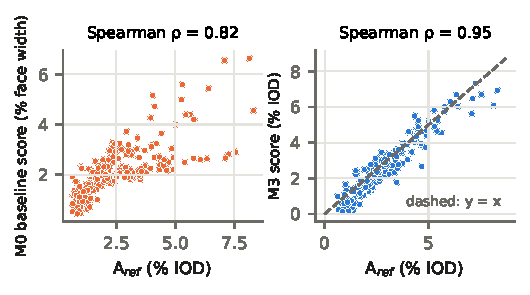
\includegraphics[width=0.7\linewidth]{agreement.pdf}
\caption{Each dot is one test face. Left: baseline. Right: ours, close to the $y=x$ line.}\end{figure}
\textbf{How to read it:} replacing \emph{only} the KD-tree matching with fixed pairs (same
detections, same midline) already raises $\rho$ from \rhoMzero{} to \rhoMzeroFixed{}. So
\emph{wrong correspondence was the baseline's main problem}. The fitted axis on the 68-point
layout gives \rhoMone{} (average error \maeMone\% IOD), and mirror averaging gives \rhoMthree{}.

\textbf{Regions and shrinkage (E3).} Regional agreement is 0.84--0.98. The detector's
asymmetry is systematically \emph{smaller} than the experts': by \shrinkGlobal\% overall and
\shrinkMouth\% at the mouth (statistically significant everywhere except the brows).
MediaPipe has a built-in ``average face'' prior that pulls unusual (asymmetric) shapes
towards symmetry. So our regional numbers should be read as conservative.

\subsection{E8: head pose dominates in-the-wild asymmetry}
\begin{figure}[h]\centering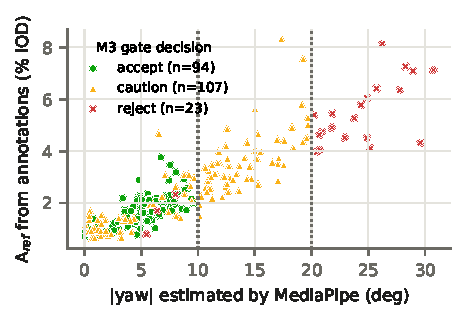
\includegraphics[width=0.55\linewidth]{pose_confound.pdf}
\caption{Asymmetry from expert landmarks against head yaw. Dotted lines: gate limits.}\end{figure}
\begin{center}\begin{tabular}{@{}lccccc@{}}
\toprule
$|$yaw$|$ (deg) & n & A$_{ref}$ & M1 & $|$err$|$ M3 & NME\\
\midrule
0-5 & 77 & 1.20 & 0.80 & 0.47 & 3.03\\
5-10 & 67 & 2.14 & 1.86 & 0.40 & 5.51\\
10-20 & 60 & 3.60 & 3.41 & 0.42 & 3.32\\
$\geq$20 & 20 & 5.50 & 5.42 & 0.57 & 4.13\\
\bottomrule
\end{tabular}
\end{center}
\textbf{How to read it:} even from expert landmarks, asymmetry rises from \yawLow\% to
\yawHigh\% as yaw grows ($\rho$ = \rhoYawRef{}). This is a property of 2D photos, not of
our detector. The detector's error (``$|$err$|$ M3'') stays about the same at every yaw. That
is exactly why a separate pose check is needed: a check that only looks at detector error
would not catch it. Among gate-accepted faces the correlation falls to \rhoYawRefAcc{}.

\begin{careful}
The pose groups contain \emph{different people} (each LFPW person appears once). Do not say
``the same face measured at different angles''.
\end{careful}

\subsection{Does the mirror test find bad landmarks?}
\begin{figure}[h]\centering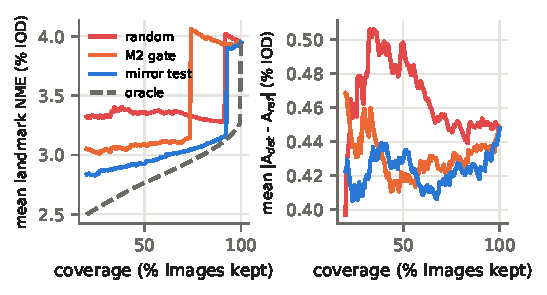
\includegraphics[width=0.62\linewidth]{risk_coverage.pdf}
\caption{Risk--coverage. Keep the images the signal trusts most; the y-axis is the average error
of the kept images (lower is better).}\end{figure}
\textbf{Risk--coverage curve:} sort images from most to least trusted by a signal and keep the
top $x$\%. A good signal keeps low-error images first. The area under the curve (AURC)
summarises it: lower is better.
\begin{itemize}
\item For landmark error (left): random \aurcRandom{}, gate signals without the mirror test
\aurcGateTwo{}, \textbf{mirror test \aurcMirror{}}, perfect oracle \aurcOracle{}. The mirror
test closes \gapClosed\% of the gap between random and perfect.
\item For the asymmetry error on clean photos (right), no signal does much better than random
(\aurcAsymMirror{} vs.\ \aurcAsymRandom{}). On clean photos, most landmark errors are similar on
both sides and cancel in $A$. The gate pays off on degraded photos (next section).
\end{itemize}

\subsection{E4--E7: robustness to degraded photos}
26 settings $\times$ 224 faces = 5{,}824 degraded images: brightness $\times$0.25 to $\times$2.5,
blur of 1--8\% of IOD, a grey box over one eye/nose/mouth, rotation $\pm$5--30$^\circ$, and
shrinking to 50--12\% of the size.
\begin{figure}[h]\centering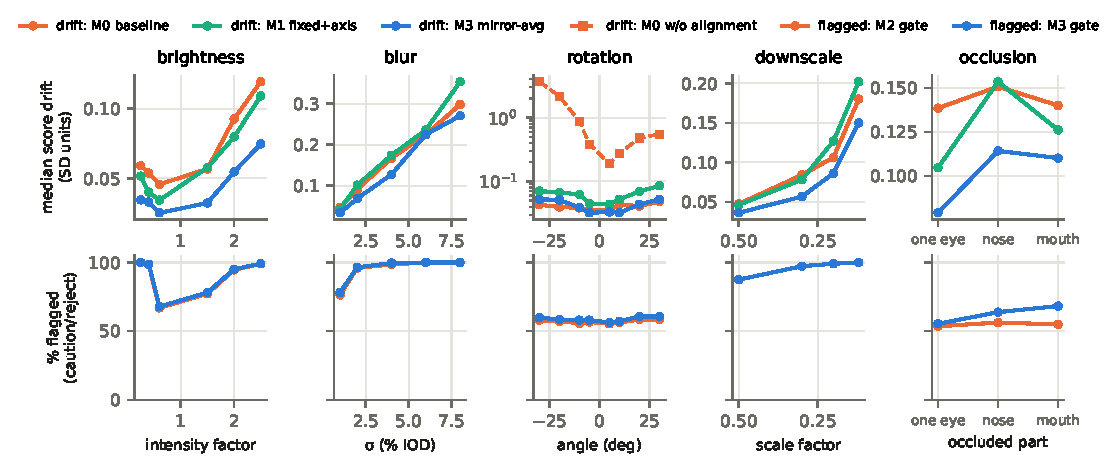
\includegraphics[width=\linewidth]{robustness.pdf}
\caption{Top: drift (lower is better). Bottom: \% of images the gate flags.}\end{figure}
\textbf{How to read it:}
\begin{itemize}
\item MediaPipe still finds a face in at least \detMin\% of images in every setting. So the
risk is not ``no answer'' but a \emph{plausible-looking wrong answer}.
\item Blue (mirror averaging) drifts least under every type of degradation.
\item Rotation panel (log scale): the vertical-midline method without alignment drifts by up to
\rotNoAlignMax{} SD. Our fitted axis stays below \rotMthreeMax{} SD with no re-detection.
\item The gate flags more and more images as blur, darkness or shrinking increase, which is what
we want.
\end{itemize}

\subsection{E9: ablation (what each component contributes)}
\begin{center}\small\begin{tabular}{@{}llcccccc@{}}
\toprule
Setting & Var. & n & Reported & Accepted & $\rho$ & Silent fail. & Drift\\
 & & & (\%) & (\%) & vs ref & (\%) $\downarrow$ & (SD) $\downarrow$\\
\midrule
Clean test & M0 & 224 & 100.0 & 100.0 & 0.823 & -- & --\\
 & M1 &  & 100.0 & 100.0 & 0.938 & 5.8 & --\\
 & M2 &  & 90.2 & 43.3 & 0.921 & 4.9 & --\\
 & M3 &  & 89.7 & 42.0 & 0.932 & 4.0 & --\\
\midrule
Perturbed, pooled & M0 & 5824 & 98.4 & 98.4 & 0.814 & -- & 0.070\\
 & M1 &  & 98.4 & 98.4 & 0.921 & 8.1 & 0.076\\
 & M2 &  & 64.0 & 22.6 & 0.918 & 3.4 & =\\
 & M3 &  & 63.2 & 21.0 & 0.927 & 3.6 & 0.054\\
\midrule
\quad blur & M0 & 1120 & 94.0 & 94.0 & 0.787 & -- & 0.131\\
 & M1 &  & 94.0 & 94.0 & 0.870 & 14.4 & 0.130\\
 & M2 &  & 37.0 & 5.8 & 0.903 & 2.7 & =\\
 & M3 &  & 35.6 & 5.2 & 0.919 & 2.3 & 0.099\\
\midrule
\quad downscale & M0 & 896 & 98.7 & 98.7 & 0.821 & -- & 0.087\\
 & M1 &  & 98.7 & 98.7 & 0.909 & 9.2 & 0.097\\
 & M2 &  & 33.5 & 4.0 & 0.919 & 1.8 & =\\
 & M3 &  & 33.4 & 4.0 & 0.927 & 1.9 & 0.066\\
\midrule
\quad brightness & M0 & 1344 & 99.5 & 99.5 & 0.818 & -- & 0.065\\
 & M1 &  & 99.5 & 99.5 & 0.936 & 5.8 & 0.056\\
 & M2 &  & 62.8 & 10.6 & 0.927 & 2.8 & =\\
 & M3 &  & 62.4 & 10.2 & 0.940 & 2.7 & 0.037\\
\midrule
\quad occlusion & M0 & 672 & 98.8 & 98.8 & 0.804 & -- & 0.142\\
 & M1 &  & 98.8 & 98.8 & 0.919 & 8.8 & 0.124\\
 & M2 &  & 87.9 & 45.1 & 0.900 & 6.2 & =\\
 & M3 &  & 85.1 & 37.5 & 0.911 & 6.0 & 0.098\\
\midrule
\quad rotation & M0 & 1792 & 100.0 & 100.0 & 0.825 & -- & 0.039\\
 & M1 &  & 100.0 & 100.0 & 0.944 & 5.2 & 0.059\\
 & M2 &  & 88.1 & 43.0 & 0.924 & 4.0 & =\\
 & M3 &  & 87.7 & 41.4 & 0.928 & 4.9 & 0.040\\
\bottomrule
\end{tabular}
\end{center}
\textbf{How to read it:} without a gate (M1), \silentPoolOne\% of degraded measurements are
silent failures (\silentBlurOne\% under blur). With the gate (M2/M3) this falls to
\silentPoolTwo\%/\silentPoolThree\% (\silentBlurThree\% under blur). The price is coverage:
only \covPoolThree\% of degraded and \covCleanThree\% of clean images still get a score. M3 has
the lowest drift (\driftPoolThree{} vs.\ \driftPoolOne{} SD).

\subsection{Gate behaviour on clean photos, and an honest negative result}
On the clean test set M3 accepts \pAccept\%, cautions \pCaution\% and rejects \pReject\%
of faces. Pose is the main trigger: LFPW faces are mostly turned. Accepted faces have a lower
landmark error (\nmeAccept\% vs.\ \nmeCaution\% NME).

\textbf{Negative result:} when a grey box covers the nose or mouth, the region is flagged
unreliable in \occNose\% and \occMouth\% of faces. When it covers an \emph{eye}, it is
flagged in only \occEye\%. MediaPipe ``invents'' the hidden eye from its average-face prior,
the same way in both the photo and its mirror, so the mirror test sees agreement. Lesson:
\emph{the mirror test catches inconsistent landmarks, not confidently invented ones.} An
appearance-based occlusion check is future work.

%======================================================================
\section{The code, file by file}
%======================================================================
\begin{center}\small
\begin{tabular}{@{}p{4.4cm}>{\raggedright\arraybackslash}p{11cm}@{}}
\toprule
File & What it does\\
\midrule
\texttt{src/fsm/detector.py} & Loads MediaPipe once; \texttt{detect(img)} returns 478 points, the pose matrix and the number of faces; \texttt{pose\_from\_transform} turns the matrix into yaw/pitch/roll.\\
\texttt{src/fsm/mesh.py} & Mirror permutation from the canonical model; the 68-point pairs and regions; the fitted 478$\to$68 map.\\
\texttt{src/fsm/geometry.py} & All the maths: reflection, fitted axis, asymmetry $a_i$, $A$, $A_r$; the baseline KD-tree method; un-flipping and mirror inconsistency.\\
\texttt{src/fsm/quality.py} & Sharpness/brightness/clipping on the face crop; \texttt{gate\_decision} (accept/caution/reject + reasons); \texttt{risk\_score}.\\
\texttt{src/fsm/pipeline.py} & \texttt{raw\_detect} (all detector calls) and \texttt{measure\_from\_raw} (all geometry); \texttt{variant\_outputs} turns one measurement into M0--M3.\\
\texttt{src/fsm/viz.py} & Drawing: mesh, axis, pairs, residuals, heatmap, status banner.\\
\texttt{src/fsm/data.py} & Reads LFPW \texttt{.pts} files; crops to the annotated face.\\
\texttt{app.py} & Streamlit interface; it only \emph{calls} the engine, with no maths in the UI.\\
\texttt{experiments/} & Run in order: \texttt{cache\_detections} $\to$ \texttt{fit\_mp68\_mapping} $\to$ \texttt{calibrate\_gate} $\to$ \texttt{run\_clean\_eval} $\to$ \texttt{run\_perturbations} $\to$ \texttt{summarize\_perturbations} $\to$ \texttt{make\_figures}, \texttt{make\_tables}.\\
\texttt{configs/} & Canonical face model, fitted map, gate limits (JSON); no thresholds are hard-coded in the UI.\\
\texttt{tests/test\_geometry.py} & 15 unit tests: reflection, zero score for a symmetric face, rotation/scale invariance, known displacement, un-flip round trip, mirror-consistent map, gate levels.\\
\bottomrule
\end{tabular}
\end{center}
\textbf{Design choices you may be asked about:} the engine never imports Streamlit, so the
same code runs the app and the experiments. Detections are cached once, so every variant
is scored on identical landmarks. Every table and figure in the paper is written by a
script from saved CSVs, so no number was typed by hand.

%======================================================================
\section{The app, screen by screen}
%======================================================================
\begin{itemize}
\item \textbf{Sidebar}: choose upload or webcam; ``stress-test'' sliders (brightness, blur,
rotation, occlusion) to show the gate reacting live; a toggle to show the baseline's number.
\item \textbf{Verdict}: green/amber/red box with the reasons (for example ``head is turned
left/right''). For reject the score shows ``withheld''.
\item \textbf{Numbers}: asymmetry $A$ (\% IOD), mirror stability $\pm$, symmetry index (0--100).
\item \textbf{Overlays tab}: mesh; fitted axis with pairs; green point vs.\ red reflection of
its twin; heatmap (grey = unreliable region).
\item \textbf{Regions tab}: table and bar chart for the five regions, with reliable/unreliable status.
\item \textbf{Quality signals tab}: each signal's value next to its caution/reject limits, and the pose angles.
\item \textbf{Export tab}: JSON and CSV download.
\end{itemize}

%======================================================================
\section{How to present it}
%======================================================================
\textbf{The story in four sentences:}
(1) Symmetry tools give a number for every photo, but 2D photos are easily dominated by
pose and image quality. (2) We measure with correct anatomical pairs and a fitted axis, check
the landmarks with a mirror test, and gate on quality and pose. (3) Against expert landmarks and
under 26 degradations, this agrees much better and prevents most silent failures. (4) We are
honest about what it cannot do: occluded eyes, shrinkage, 2D pose.

\textbf{Suggested split} (change to match who actually did what):
slides 1--5 Pankaj; 6--9 Prutha and Ashish; 10--14 Ankit and Ashish; 15 Pankaj;
16 (demo) Mahi; 17 Prutha. The speaker notes on every slide hold the details, and
\texttt{presentation/DEMO\_SCRIPT.md} has the step-by-step demo.

\textbf{Timing for about 12 minutes:} problem and motivation 2 min; related work and
contributions 1.5 min; method 3 min; results 3 min; failures 1 min; demo 2--3 min.

%======================================================================
\section{Questions you should be ready for}
%======================================================================
\begin{description}[style=nextline,leftmargin=0pt,itemsep=5pt]
\item[What exactly is novel?] Not landmarks, regions or the UI; those exist. Our novelty is
(1) fixed anatomical pairs plus a fitted axis, which fixes the \kdWrong\% wrong-partner
problem and raises agreement from \rhoMzero{} to \rhoMthree{}; (2) the mirror test as a
label-free reliability signal and bias-cancelling average; (3) a train-calibrated gate
evaluated by silent failures and coverage; (4) the evaluation protocol.
\item[How do you know your score is right without labels?] We compare with the identical
measure on expert landmarks, and we use degradations where the answer is known not to
change. We do not claim agreement with human symmetry \emph{ratings}; we have none.
\item[Why not just align the face like the baseline?] Alignment needs a second detection
and still relies on two points being correct. The fitted axis is mathematically
rotation-invariant and uses all 51 inner points.
\item[Why IOD and not face width?] IOD is the 300-W standard and does not depend on the jaw
outline, which moves with pose.
\item[Did you tune thresholds on the test set?] No. Pose and size limits were set a priori;
the rest are training-set percentiles. The test set was only evaluated.
\item[Why does the gate reject so many LFPW faces?] LFPW is in-the-wild: about two thirds of
test faces are turned more than 5$^\circ$. Given $\rho$ = \rhoYawRef{} between yaw and
asymmetry, refusing those is correct behaviour.
\item[Why not train a deep network?] There are no symmetry labels to train on, and explicit
geometry is interpretable and unit-testable. Training a detector was out of scope.
\item[Could MediaPipe have seen LFPW in training?] Possibly; its training data is not public.
That is why we do not present its NME as an independent benchmark result, only as a
comparison between our mappings and signals.
\item[What is the 0--100 index?] A monotone re-expression of $A$ for readability, with the
median training face at 50. It is not a validated scale.
\item[Is this a medical or attractiveness score?] No. It is a 2D geometric indicator, and the
app says so.
\item[Did you copy code?] No. The audited repositories have no licence, so we
re-implemented the baseline method ourselves. The MediaPipe model and canonical mesh are
Apache-2.0.
\item[What would you do next?] Use MediaPipe's 3D landmarks to undo yaw and validate on
AFLW2000-3D (which has true pose); add an appearance-based occlusion check; use WFLW subsets;
collect consented multi-pose photos with human symmetry ratings.
\end{description}

%======================================================================
\section{Glossary}
%======================================================================
\begin{description}[leftmargin=0pt,itemsep=1pt]
\item[$A$ / $A_r$] global / regional asymmetry, in \% IOD.
\item[$A_{ref}$] the same measure computed from expert landmarks (the reference).
\item[AURC] area under the risk--coverage curve; lower is better.
\item[Bilateral pair] a point and its mirror twin on the other side of the face.
\item[Canonical face model] MediaPipe's exactly symmetric 3D average face.
\item[Caution / reject] the gate's warning level / refusal level.
\item[$\delta$, $\delta_r$] mirror inconsistency (whole inner face / one region), as a fraction of IOD.
\item[Drift] median score change under degradation, in units of the between-person SD.
\item[IOD] inter-ocular distance (outer eye corner to outer eye corner).
\item[KD-tree] a data structure for fast nearest-neighbour search; the baseline uses it to match points.
\item[LFPW / 300-W] the benchmark with 68 expert landmarks per face that we used.
\item[M0--M3] baseline, fixed pairs + axis, + gate, full system.
\item[NME] landmark error divided by IOD.
\item[$\pi$] the mirror permutation: $\pi(i)$ is the twin of point $i$.
\item[Silent failure] a reported score that is off by more than 1\% IOD.
\item[Yaw / pitch / roll] turning left--right / nodding / tilting to a shoulder.
\end{description}


\end{document}
